% !TeX root = logicNotes.tex

\chapter{Introduction to Propositional Logic}
\section{Declarative statements}
We are interested in creating a language in which mathematical proofs can be written. The language should be simple enough so that vague and unambiguous statements cannot be written. On the other hand, it should be powerful enough for proofs to be written. We will build a language in which all of mathematics can be embedded. We begin with propositional logic, the foundation on which other logics are built on.

We say that \emph{true} and \emph{false} are \emph{boolean values}. They will be denoted by the symbols \true\/ and \false\/ respectively. \indexit{Declarative sentences} are statements which can be assigned either true or false. For example,
\begin{enumerate}
\item 179179 is a composite number.
\item Sun rises in the east and Japan is in Europe
\item Kattapa killed Bahubali.
\item P = NP
\item John Snow's father is Ned Stark
\end{enumerate}
Since the number 179179 is divisible by 7,11,13 and 179, statement (1) is true. On the other hand statement (2) is false since Japan is not in Europe. Statement (3) is true. We do not yet know whether Statement (4) is true or false but the statement as such can be assigned true or false. Statement (5) is true or false depending on till which episode you have watched game of thrones. 

The following statements are not declarative 	
\begin{enumerate}
\item What is the time?
\item Submit your assignments today.
\item Teek Hai!
\end{enumerate}

Some declarative statements can be thought of as \indexit{atomic}. That is, those statements cannot be further split into logical sentences. In the above example Statement (2) is not atomic because it can be split into sentences ``Sun rises in the east'' and ``Japan is in Europe''.

\section{Propositions}
As mathematicians we are not interested in the information contained in the declarative sentences. That is, we are not interested whether ``Kattapa killed Bahubali" or ``Sun rises in the east" in the real world. Rather we are interested in only whether the statements are true or false and what other statement can we understand from them. For example, consider the following statement.

\myquote{``If it rains in Delhi today, you will fail in logic course."}

This is a weird statement but the statement is a declarative statement. That is, it can either be true or false. To summarize the point being made. We are not really interested in the weirdness or the reality of the real world. We are only interested in statements which can be assigned boolean values. Hence we map declarative sentences to symbols. We will denote atomic sentences using symbols $p,q,r,\dots$ or $p_1,p_2,\dots$. These will be termed as \indexit{propositions} and the logic we build using propositions as \emph{propositional logic}. We will also denote true by \true\/ and false by \false.

Propositions can be modified/combined using certain symbols called \indexit{logical connectives}. This way we can build complex logical statements. The logical connectives we will be interested in and their \indexit{semantics} follow
\paragraph{Negation} \index{negation} For any sentence, its negation is the opposite of it. For example, the negation of ``Kattapa killed Bahubali'' is ``Kattapa did not kill Bahubali''. Similarly negation of ``P=NP'' is ``P $\neq$ NP''. The negation of a propositional symbol, $p$ is denoted as $\neg p$ (and called negation of $p$). If the $p$ is true then $\neg p$ is false. On the other hand, if $p$ is false, $\neg p$ is true. The following \indexit{truth table} summarizes the semantics of negation.

\begin{table}[ht]
\centering
\begin{tabular}{c|c}
$p$ & $\neg p$ \\
\hline
\true & \false \\
\false & \true \\
\end{tabular}
\caption{Truth table for negation}
\end{table}

\paragraph{Conjunction} \index{conjunction} stands for \emph{and}. When it is used to connect two declarative sentences it means that both the sentences are true. 
For example, ``$2$ is a prime number'' and ``$2$ is an even number''. We use the symbol $\wedge$ to denote and. The following truth table captures the meaning of $\wedge$.

\begin{table}[H]
\centering
\begin{tabular}{c|c|c}
$p$ & $q$ &$p \wedge q$ \\
\hline
\true & \true & \true \\
\true & \false &  \false \\
\false & \true & \false \\
\false & \false & \false 
\end{tabular}
\caption{Truth table for conjunction}
\end{table}


\paragraph{Disjunction} \index{disjunction} stands for \emph{or}. Disjunctions are slightly different from the or we use in English (or most natural languages). Assume that I made the following announcement in class.

\myquote{``Tomorrow there will be a lecture or an exam."}

It is natural for you to assume that there will either be a lecture tomorrow and no exam, or there will be an exam and no lecture. That is, you would never think of the possibility of both a lecture and an exam going to be held tomorrow. But, or used in a mathematical sentence, can mean both of them happening. This is the difference of disjunction in or in logic and natural language. We have a name for the or in natural language. We call it xor and is denoted by the symbol $\xor$. See Exercise \ref{exercise:xor}. Coming back to disjunction in logic, the symbol for or is $\vee$ and its semantics is given by the following truth table.
\begin{table}[H]
\centering
\begin{tabular}{c|c|c}
$p$ & $q$ &$p \vee q$ \\
\hline
\true & \true & \true \\
\true & \false &  \true \\
\false & \true & \true \\
\false & \false & \false 
\end{tabular}
\caption{Truth table for disjunction}
\end{table}
The semantics for xor is given below.

\begin{table}[ht]
\centering
\begin{tabular}{c|c|c}
$p$ & $q$ &$p \xor q$ \\
\hline
\true & \true & \false \\
\true & \false &  \true \\
\false & \true & \true \\
\false & \false & \false 
\end{tabular}
\caption{Truth table for xor}
\end{table}


\paragraph{Implication} \index{implication} is used to state a necessary condition. It is denoted by the symbol $\ifthen$. The statment 
\myquote{If $x$ is prime, then $x \neq 4$}
 is an example of an implication. Typically it is written in the form ``If $p$ then $q$'' and in propositional logic as $p \ifthen q$.  Its truth table is given in Table \ref{tab:implication}.
\begin{table}[ht]
\centering
\begin{tabular}{c|c|c}
$p$ & $q$ &$p \ifthen q$ \\
\hline
\true & \true & \true \\
\true & \false &  \false \\
\false & \true & \true \\
\false & \false & \true 
\end{tabular}
\caption{Truth table for implication}
\label{tab:implication}
\end{table}
We will explain the truth table with an example. Consider the statement 

\myquote{``If you work hard, you get good grades''. }

The statement is true if you work hard and got good grade. On the other hand it is false if you work hard and did not get good grades. The tricky question is, what if you did not work hard and got good grades. Does this violate our the statement? No, it doesnt and hence we can assign the statement to be true in this case also. Similarly the statement is true, if we did not work hard and did not get good grades.

Implication is a little tricky to understand especially for beginners. The following puzzle helps you to understand it better.
\begin{puzzle}[Wason]
The following cards are kept on the table. Each card has a letter on one side and a number on the other side.
\begin{figure}[h]
\centering

\includegraphics[width=8cm]{ak47.jpg}
\end{figure}
We make the following claim: ``If a card has a vowel on one side, then it has an even number on its opposite side". Which cards must one flip to check if the claim is correct?
\end{puzzle}
\begin{solution}
The answer is cards $A$ and $7$. Let us look at each of the card and check whether we need to flip or not. Card A has to be flipped, because we need to be sure that on the opposite side is a vowel. Card K need not be checked. Why? Because, it does not matter to us if, the opposite side has an even number or odd number. Similarly we do not have to flip $4$ since it does not matter to us whether the opposite side was vowel or consonant. On the other hand, card $7$ has to be flipped because we have to make sure it is not a vowel on the other side. Because if there was a vowel, we would have violated the claim.
\end{solution}

\section{Formulas}
By repeatedly using logical connectives we can make complex declarative statements. For example, 

\myquote{If $x$ is prime and $x \neq 2$,  then $x$ is odd}

is a statement made by first conjuncting two statements ``$x$ is prime" and ``$x \neq 2$". It is then used in implication with statement ``$x$ is odd". In propositional logic this statement can be wrriten as follows
\myquote{$($``$x$ is prime" $\wedge$ ``$x \neq 2$"$) \ifthen$ ``$x$ is odd"}
Such complex statements in logic are called \indexit{formulas}. We denote propositional formulas by greek letters like $\alpha, \beta, \gamma, \dots$ etc or $\alpha_1, \alpha_2, \dots$.
\begin{definition}
A {formula} is inductively constructed using the following rules (and no other rules)
\begin{enumerate}
\item A proposition is a formula
\item If $\alpha$ and $\beta$ are formulas then $\neg \alpha$, $\alpha \vee \beta$, $\alpha \wedge \beta$, $\alpha \ifthen \beta$ are formulas
\end{enumerate}
\end{definition}
We can write truth tables for formulas by inductively building the table. Consider the following formula and its truth table $$\alpha \defs \big((p \ifthen \neg q) \ifthen (q \vee \neg p)\big)$$.
\begin{table}[H]
\centering
\begin{tabular}{c|c|c|c|c|c|c}
$p$ & $q$ &$\neg p$ & $\neg q$ & $p \ifthen \neg q$ & $q \vee \neg p$ & $\alpha$ \\
\hline
\true & \true & \false & \false & \false & \true & \true \\
\true & \false &  \false & \true & \true & \false & \false \\
\false & \true & \true  & \false & \true & \true & \true \\
\false & \false & \true & \true & \true & \true & \true
\end{tabular}
\caption{Truth table for $\alpha \defs \big((p \ifthen \neg q) \ifthen (q \vee \neg p)\big)$}
\end{table}


For a formula $\alpha$ with propositions $p_1,p_2,\dots, p_n$, a \indexit{valuation} is a particular \true/\false\/ assignment to the propositions $p_1,\dots, p_n$. That is a valuation, $v: \{p_1,p_2,\dots,p_n\} \rightarrow \{\true, \false\}$ is a function from the propositions to boolean values. Note that, there are $2^n$ different valuations possible for $n$ propositions.
\begin{example}
Consider the formula $p \wedge q$. One particular valuation is $p$ is assigned \true\/ and $q$ is assigned \false. The formula is evaluated to false for this valuation.
\end{example}

%\section[Types of Formulas]{Types of Formulas: Tautology, Contradiction, \dots}
We say that two formulas are \indexit{equivalent} if they have the same truth table. It will be denoted by the symbol $\equiv$. \index{$\equiv$} 

\begin{example}
If and only if (written also as \indexit{iff}) is used to denote a necessary and sufficient condition. In symbolic form it is denoted by $\ifonlyif$. Semantically $p \ifonlyif q$ is equivalent to $p \ifthen q$ and $q \ifthen p$. The truth table is given below.
\begin{table}[H]
\centering
\begin{tabular}{c|c|c}
$p$ & $q$ &$p \ifonlyif q$ \\
\hline
\true & \true & \true \\
\true & \false &  \false \\
\false & \true & \false \\
\false & \false & \true 
\end{tabular}
\label{tab:iff}
\caption{Truth table for if and only if}
\end{table}
\end{example}

Here is another example which introduces the \indexit{contrapositive} of an implication. The formula $(\neg q \ifthen \neg p)$ is the {contrapositive} of the statement $p \ifthen q$. The following exercise shows that an implication and its contrapositive are equivalent.
\begin{exercise}
Show that the following formulas are equivalent.
\begin{enumerate}
\item $p \ifthen q$
\item $(\neg q \ifthen p)$
\item $\neg p \vee q$
\end{enumerate}
What is the complement of $p \ifthen q$?
\label{exercise:implequiv}
\end{exercise}


\begin{exercise}[DeMorgan's law]
\label{exercise:demorgansem}
Show that $p \wedge q  \equiv \neg (\neg p \vee \neg q)$ and  $p \vee q  \equiv \neg (\neg p \wedge \neg q)$
\end{exercise}

The following exercise connects xor and disjunctions.
\begin{exercise}
\label{exercise:xor}
Write a formula using only the symbols disjunctions and negations which is equivalent to $p \xor q$.
\end{exercise}

\begin{exercise}
Consider you are given a truth table with propositions $p_1,\dots,p_n$. Give an algorithm which outputs a formula (using only symbols $\vee,\wedge, \neg$) having the same truth table.
\end{exercise}

The above exercise (along with demorgan's law) show that any formula can be converted into an equivalent formula which uses only the symbols $\wedge$ and $\neg$.

\begin{exercise}
Convert any formula into an equivalent formula which uses only symbols $\wedge$ and $\neg$.
\end{exercise}

We say that a formula $\alpha$ is \indexit{satisfiable} if there is a valuation which makes $\alpha$ true. In other words, $\alpha$ is satisfiable if we can find atleast one \true\/ in the column for $\alpha$ in the truth table of $\alpha$. A formula $\alpha$ is a \indexit{tautology} if for all valuations $\alpha$ is true. In other words $\neg \alpha$ is not satisfiable. On the other hand, $\alpha$ is a \indexit{contradiction} or \indexit{unsatisfiable} if $\alpha$ is not satisfiable. That is $\neg \alpha$ is a tautology.
\begin{exercise}
\begin{enumerate}
\item Give a formula which is a tautology?
\item Give a formula which is satisfiable but not a tautology?
\item Give a formula which is a contradiction?
\end{enumerate}
\end{exercise}

\section[Encoding using logic]{Application of Logic: Encoding problems}
We use propositional logic to encode different problems.

\subsection{Digital circuits}
\begin{exercise}
We can view a proposition being assigned to $1$ or $0$ (in place of \true\/ or \false). That is a proposition $p$ can be thought of as a bit variable. Extending the idea, a valuation to a $n$ proposition symbols can be thought of as an $n$-bit number. Use this view to write a formula to encode addition relation between two $n$-bit numbers. That is, write a formula which satisfies the following condition
\begin{align*}
p_1p_2\dots p_n  \\
+ \\
q_1q_2 \dots q_n &  \\
= \\
r_1r_2 \dots r_n
\end{align*}
View $p_1,\dots,p_n,q_1,\dots,q_n,r_1,\dots,r_n$ as propositions.
\end{exercise}

\subsection{Mathematical statements}
\begin{exercise}[Pigeon hole principle]
If $n+1$ pigeons are placed on $n$ holes, atleast one hole will have more than one pigeon. This is the pigeon hole principle. Now, consider $n+1$ pigeons and $n$ holes. Let proposition $p_{i,j}$ denote the fact that the $i^{th}$ pigeon is in the $j^{th}$ hole.  Write a propositional logic formula to encode the pigeon hole principle. 
\end{exercise}


\subsection{Puzzles}
\begin{exercise}[Smullyan]
Use propositional logic to answer the following questions
\begin{enumerate}
\item You are trapped in a room. There are two doors. Either the doors lead to an exit or to a lion (note that both leading to an exit or to a lion are also possible). In Door 1, it is written ``This door is exit and other door leads to lion". In Door 2, it is written ``One of the rooms lead to exit, the other to a lion". You are told that only one of the written statements are true and the other false. Which door would you choose?
\item Similar to the previous question. You are trapped in a room. There are two doors. Either the doors lead to an exit or to a lion (note that both leading to an exit or to a lion are also possible). In Door 1, it is written ``Atleast one of the doors is an exit". In Door 2, it is written ``There is a lion on the other door". You are told that either both are true statements or both are false. Which door would you choose?
\item One more question with same flavour. You are trapped in a room. There are two doors. Either the doors lead to an exit or to a lion (note that both leading to an exit or to a lion are also possible). In Door 1, it is written ``This door is exit or the other door leads to lion". In Door 2, it is written ``The exit is the other door". The statements are either both true or both false. Which door would you choose?
\end{enumerate}
\end{exercise}

\begin{exercise}[Smullyan]*
Can you think of encoding the following problem in propositional logic such that it has a solution iff the formula is satisfiable.
\begin{figure}[H]
\centering
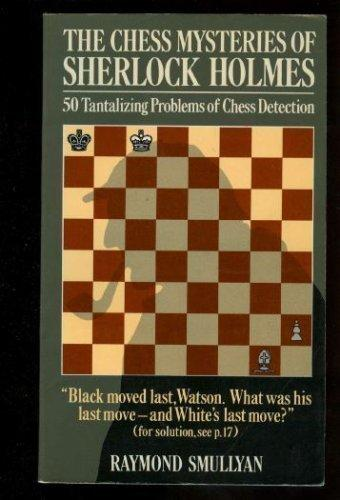
\includegraphics[width=5cm, height=5cm]{chess.jpg}
\end{figure}
The reader is expected to understand how to go about doing this. He/she is not expected to write the entire formula (which is going to be very big).
\end{exercise}

\begin{exercise}[Indian Puzzle championship 2010]*
Fill in the grid in such a way that every row and every column contains numbers from $(1-5)$ exactly once. Some cells may remain blank. The numbers inside the grid represent the height of
the building in the corresponding cell. The numbers outside the grid represent the number of buildings visible from that direction.
\begin{figure}[H]
\centering
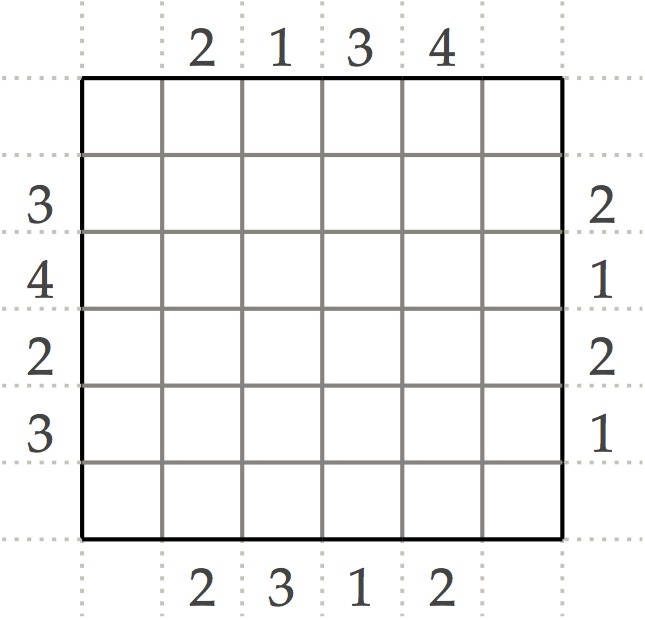
\includegraphics[width=5cm,height=5cm]{skyscrapper.jpg}
\end{figure}

Encode the problem in propositional logic.
\end{exercise}

\section{Satisfiability of propositional formulas}
How hard is it to check whether a propositional formula is satisfiable?  

\begin{problem}
\caption*{{\bf Problem} SAT}
{\bf Input: } A propositional formula $\alpha$ \\
{\bf Output: } YES if $\alpha$ is satisfiable, otherwise NO
\label{prblm:sat}
\end{problem}

For a formula $\alpha$ with $n$ propositions the truth table has $2^n$ number of rows. Therefore building the truth table and checking each row is a trivial way to check for satisfiability. This algorithm though takes exponential time, since the number of rows in the truth table is $2^n$. 
In other words, $O(2^n)$ is an upper bound for checking satisfiability of a formula with $n$ propositions. The interesting question is, does there exist a faster algorithm. Or even better, does there exist a polynomial time algorithm. That is, an algorithm whose number of steps is $O(n^c)$ for some constant $c$. It turns out, we do not yet know the answer to this question. Most computer scientists think there is no polynomial time algorithm for SAT. The problem is NP-complete (in NP and is NP-hard) and hence finding a polynomial time algorithm is equivalent to answering P=NP. 

\begin{exercise}
\label{exercise:satisnp}
Show that SAT is in NP? 
\end{exercise}

To show that SAT is NP-hard, we need to reduce from an NP-complete problem into SAT. The next exercise asks you to reduce from the Hamiltonian problem.

\begin{exercise}
\label{exercise:satisnphard}
Give a polynomial time algorithm which takes as input a graph $G=(V,E)$ and outputs a propositional formula $\alpha$ such that the graph has a Hamiltonian cycle if and only if $\alpha$ is satisfiable. Does the valuation which makes $\alpha$ true give us the cycle? [A Hamiltonian cycle is a cycle which traverses every vertex exactly once.]
\end{exercise}

Now assume that we do not know that Hamiltonian cycle is NP-complete. Can you argue from the definition of NP-hardness? We need to show that there is a reduction from every NP problem into SAT. 

\begin{exercise}
Given a non-deterministic Turing Machine which runs in $poly(n)$ time (say in time $n^2$) and an input of size $n$, construct a propositional logic formula (of size polynomial in $n$) such that the formula is satisfiable if and only if the Turing machine accepts the input.
\end{exercise}

The following theorem is a consequence of our discussion until now.
\begin{theorem}
SAT is NP-complete.
\end{theorem}
\begin{proof}
A problem is NP-complete if it is both in NP and is NP-hard. It follows from Exercise \ref{exercise:satisnp} and Exercise \ref{exercise:satisnphard} that SAT is NP-complete.
\end{proof}

%\section{CNF and satisfiability}
A \indexit{literal} is either a proposition or a negation of a proposition. That is, it is of the form $p$ or $\neg p$, where $p$ is a proposition. A \indexit{clause} is a literal or a disjunction of literals. A \indexit{CNF formula} is a conjunction of clauses. Consider the following problem.

\begin{problem}
\caption*{{\bf Problem} CNF SAT}
{\bf Input: } A CNF formula $\alpha$ \\
{\bf Output: } YES if $\alpha$ is satisfiable, otherwise NO
\label{prblm:cnfsat}
\end{problem}

The set of all CNF formulas is a subset of the set of all propositional formulas. Hence CNF-SAT is also in NP. It is a different matter that it is also NP-hard. We will give a reduction from SAT to CNF SAT.
\begin{theorem}
CNF-SAT is NP-hard.
\end{theorem}
\begin{proof}
We will give a reduction from SAT to CNF SAT. Let $\alpha$ be a propositional formula. Our aim is to give a CNF formula $\hat \alpha$ such that $\alpha$ is satisfiable if and only if $\hat \alpha$ is satisfiable. We first replace subformulas of the from $(\beta \ifthen \gamma)$ in $\alpha$ by $(\neg \beta \vee \gamma)$. The second step is to push the negations to the propositions using De-Morgan's law. That is subformulas of type $\neg (\gamma \vee \beta)$ is replaced by $\neg \gamma \wedge \neg \beta$. Similarly, $\neg (\gamma \wedge \beta)$ is replaced by $\neg \gamma \vee \neg \beta$. This is done inductively until all negations apply to propositions. We now need to convert the formula into a conjunction of disjunctions. To convert subformulas of the form $(\beta \wedge \gamma) \vee \psi$ we introduce a new proposition $p$ (which is not present in the formula). We then replace $(\beta \wedge \gamma) \vee \psi$ by $(\psi \vee p) \wedge (\beta \vee \neg p) \wedge (\gamma \vee \neg p)$. It is easy to see that the two formulas are equivalent with respect to satisfiability. Inductively applying this translation will give us a CNF formula.
\end{proof}


We will now look at special CNF formulas. A $k$-CNF formula \index{k-CNF} \index{2-CNF}  is a conjunction of clauses with at most $k$-literals. For example, the following is a $2$-CNF formula 
\[
(p \vee \neg q) \wedge (\neg r \vee s) \wedge (t \vee q) \wedge \neg t
\]
It is also a $k$-CNF formula for all $k \geq 2$. On the other hand, this is not a $2$-CNF formula because it has a disjunction of $3$ literals.
\[
(p \vee q \vee \neg r)
\]
The above formula though is a $3$-CNF formula. The set of all $3$-CNF formulas is a subset of the set of all CNF formulas. Hence $3$-CNF SAT is also in NP. 

\begin{problem}
\caption*{{\bf Problem} $3$-CNF SAT}
{\bf Input: } A $3$-CNF formula $\alpha$ \\
{\bf Output: } YES if $\alpha$ is satisfiable, otherwise NO
\label{prblm:3cnfsat}
\end{problem}

The following exercise asks you to show that $3$-CNF SAT is NP-hard. 
\begin{exercise}
Show that $3$-CNF SAT is NP-hard.
\end{exercise}

In short we have that SAT, CNF SAT and $3$-CNF SAT are all NP-complete, since they are in NP and are NP-hard. It is reasonable to assume that there does not exist polynomial time algorithms for NP-complete problems. Therefore we search for fragments of CNF whose satisfiability can be checked in polynomial time. The next two sections look at fragments which give linear time satisfiability algorithms.

\section{Semantic entailment}
In the previous sections, we saw the semantics of formulas. The truth table of a formula tells us for what valuation makes the formula true or false. In this section, we are interested in a relationship between formulas. Let us first define \indexit{semantic entailment} in its simpler form. Consider two formulas $\alpha$ and $\beta$. 

\begin{definition}
We say that $\alpha$ semantically entails $\beta$ by the following notation.
\[
\alpha \models \beta
\]
It means that, for all valuations which make $\alpha$ true, $\beta$ is also evaluated to true. 
\label{def:semantic}
\end{definition}

We can see semantic entailment in a non-mathematical setting as follows: In all the worlds where $\alpha$ is true, $\beta$ is also true. Let us look at an example
\[
\text{Planets have mass } \models \text{ There is gravity in planets}
\]
The example says that: Consider a world where planets have mass. Then planets will also show gravity. In short, ``Planets have mass" semantically entails the statement ``There is gravity in planets". This is a fact of the universe we live in. The above example was used to press the meaning of $\models$ and is not really a good example for mathematicians. 

Mathematicians require precise definitions like definition \ref{def:semantic}. Below we generalise this. Let $\Gamma$ be a set of formulas and $\beta$ a formula. Then 
\[
\Gamma \models \beta
\]
denotes that for all valuations which make all formulas in $\Gamma$ true, we have $\beta$ is true. Let us understand when $\Gamma$ is finite. That is $\Gamma = \{\alpha_1,\alpha_2,\dots,\alpha_n\}$ for some $n \in \Nat$. We take a little liberty in writing $\{\alpha_1,\alpha_2,\dots,\alpha_n\} \models \beta$ as
\[
\alpha_1,\alpha_2,\dots,\alpha_n \models \beta
\]
That is, we skip the set notation when it is clear to the reader. The following exercises show the relation between semantic entitlement in the finite case and the implication relation.

\begin{exercise}
Show that the following statements are equivalent.
\begin{enumerate}
\item $\alpha \models \beta$
\item \true $~\models (\alpha \ifthen \beta)$
\end{enumerate}
\end{exercise}

\begin{exercise}
Extend the argument in the previous exercise, and show that the following statements are equivalent.
\begin{enumerate}
\item $\alpha_1,\alpha_2,\dots,\alpha_n \models \beta$
\item \true $~ \models \Big(\alpha_1 \ifthen \big(\alpha_2 \ifthen \dots (\alpha_n \ifthen \beta)\big)\Big)$
\item \true $~\models (\alpha_1 \wedge \alpha_2 \wedge \dots \alpha_n) \ifthen \beta$
\end{enumerate}
\label{exercise:semequiv}
\end{exercise} 

Let us go back to the case when $\Gamma$ is infinite. There does not exist equivalent definitions like those in Exercise \ref{exercise:semequiv}. This is because infinite implication or conjunction is not allowed in our logic.

There is one tricky case, we will elaborate on. Consider an arbitrary formula $\alpha$. Then 
\[
\false \models \alpha 
\]
Let us go through the definition of semantic entailment. It says that for all valuations which make the left hand side (here it is \false\/) true, we have that $\alpha$ is true. This is correct, since there is no valuation which makes $\false$ true. In other words, since there is no valuation which make $\false$ true, the statement is \indexit{vacuously true}. What this means is that $\false \models \neg \alpha$ and $\false \models \alpha$. In short, if falsity is true, then anything is true.

\section{Compactness*}
We say that a set $\Gamma$ (finite or infinite) of propositional formulas is satisfiable if there is a valuation which makes all formulas in $\Gamma$ true. The following exercise answers, when is a finite set satisfiable.
\begin{exercise}
A finite set $\Gamma = \{\alpha_1,\alpha_2,\dots,\alpha_n\}$ is satisfiable if and only if $\bigwedge_{i=1}^n \alpha_i$ is satisfiable.
\end{exercise}
The interesting question is, when is an infinite set satisfiable? The compactness theorem says that if a set is unsatisfiable, then there is a finite set which is unsatisfiable. 
\begin{theorem}[Compactness]
\label{thm:propCompactness}
$\Gamma$ is satisfiable if and only if for all finite subsets $Y \subseteq \Gamma$, $Y$ is satisfiable.
\end{theorem}
\begin{proof}
The forward direction of the proof is easy to see. Let us therefore show the other direction. We assume $\Gamma$ is unsatisfiable and identify a finite set which is unsatisfiable. Let us first enumerate the propositions used by the formulas in $\Gamma$ as
\[
p_1,p_2,\dots 
\]
We add a new proposition $p_0$ (this is added just for ease of explanation and is not fundamental to the proof) to this list. Now, we build an complete binary tree where every node in the tree corresponds to a valuation for some finite set of propositions. To be precise, a node at height $t$ in the tree corresponds to a valuation for all propositions $\{p_0,p_1,\dots,p_t\}$. 
In short every node at height $t$ corresponds to a function $v: \{p_0,p_1,\dots,p_t\} \rightarrow \{\true,\false\}$. We will inductively define the valuation corresponding to every node. The root node (at height $0$) corresponds to the function $v:\{p_0\} \rightarrow \{\true,\false\}$, such that $v(p_0) = \true$. Consider an arbitrary node at height $t$ with valuation $v:\{p_1,\dots,p_t\} \rightarrow \{\true,\false\}$. The valuation of its children extends $v$ as follows. The left node corresponds to the valuation $v_l:\{p_1,\dots,p_{t+1}\} \rightarrow \{\true,\false\}$ where $v_l(p_{t+1}) = \true$ and for all other propositions $p_i$ where $i\leq t$, $v_l(p_i) = v(p_i)$. Similarly the right node corresponds to $v_r:\{p_1,\dots,p_{t+1}\} \rightarrow \{\true,\false\}$  such that $v_r(p_{t+1}) = \false$ and for all other propositions $p_i$ where $i\leq t$, $v_r(p_i) = v(p_i)$. 

We now trim the above infinite tree as follows. Take a formula $\alpha \in \Gamma$. If a valuation $v$ does not satisfy $\alpha$, then remove all descendants of the node corresponding to $v$ (but keep the node $v$). Note that, if $v$ does not satisfy $\Gamma$ then any extension of $v$ also does not satisfy $\Gamma$. We do the above trimming for all formulas $\alpha \in \Gamma$. We claim that, the trimmed tree is a finite tree. Assume not. Then there exists an infinite path in the tree. We claim that this represents a valuation $v:\{p_1,p_2,\dots \} \rightarrow \{\true,\false\}$ which satisfies all formulas in $\Gamma$. Assume not. Then there exists a formula $\alpha \in \Gamma$ such that $v$ does not satisfy $\alpha$. Let $\alpha$ be over propositions $\{p_1,\dots,p_t\}$. There is a valuation $v':\{p_1,\dots,p_t\} \rightarrow \{\true,\false\}$ which extends to $v$, such that $v'$ does not satisfy $\alpha$. This leads to a contradiction. Hence the trimmed tree is a finite tree.

Let $V = \{v_1,v_2,\dots,v_k\}$ be the set of all valuations in the leaf of the trimmed tree. Therefore any valuation $v$ extends atleast one of the $v_i$s in $V$. Now, for each $v_i \in V$ we pick one $\alpha _i\in \Gamma$ such that $v_i$ does not satisfy $\alpha_i$. Call this set $Y=\{\alpha_1,\alpha_2,\dots,\alpha_k\}$. We claim $Y$ is not satisfiable. Assume not. Then there exists a valuation $v:\{p_0,\dots,p_t\} \rightarrow \{\true,\false\}$ which satisfies $Y$ and $t$ is the height of the trimmed tree. Since the tree is finite there is an extension $v_i$ of $v$ which does not satisfy formula $\alpha_i \in Y$. This is a contradiction, since if $v_i$ satisfies $\alpha_i$, its extension $v$ should also. Hence, we have a finite set $Y$ which is not satisfiable.
\end{proof}

\section{Exercises}
\begin{exercise}
Which of the following are correct?
\begin{multicols}{2}
\begin{enumerate}
\item $p \vee q \models p$
\item $\neg q, p \vee q \models p$
\item $(p \ifthen q) \models (\neg q \ifthen \neg p)$
\item $p \ifthen q, s \ifthen t \models (p \vee s) \ifthen (q \wedge t)$
\item $(p \ifthen q) \wedge (p \ifthen r) \models p \ifthen (q \wedge r)$
\item $p \wedge \neg p \models (r \ifthen q)$
\end{enumerate}
\end{multicols}
\end{exercise}

\begin{exercise}
What can we say about the following?
\begin{multicols}{2}
\begin{enumerate}
\item \true $~ \models \alpha$
\item \true $~ \not \models \alpha$
\end{enumerate}
\end{multicols}
\end{exercise}


\begin{exercise}[Nyayasutra]
Are the following arguments correct? Write the statements using entails.
\begin{enumerate}
\item If there is smoke, then there is fire. There is smoke on hill. Therefore, there is fire. 
\item Fire causes smoke. There is smoke on hill. Therefore, there is fire.
\item If there is smoke, then there is fire. There is no smoke. Therefore, there is no fire.
\end{enumerate}
\end{exercise}

\begin{exercise}[\cite{decidability}]
Let $S = \{s_1, \dots , s_n\}$ be a set of radio stations. Let $F = \{f_1,\dots,f_k \}$ be a set of frequencys. Let $E$ be the set of pairs of stations which are close to each other. Write the following constraints in propositional logic. To model this problem, define a set of propositional variables $\{x_{ij} ~|~ i \in \{1,...,n\},j \in \{1,...,k\}\}$. Intuitively, variable $x_{ij}$ is set to true if and only if station $i$ is assigned the frequency $j$. 
\begin{enumerate}
\item Every station is assigned at least one frequency.
\item Every station is assigned not more than one frequency.
\item Close stations are not assigned the same frequency.
\end{enumerate}
\end{exercise}

\begin{exercise}[\cite{decidability}]
Are these two programs equivalent? Explain why you think so.
\begin{figure}[H]
\centering
\begin{tabular}{|p{55mm}|p{55mm}|}
\hline
if $(!a ~\&\& ~!b)$ h(); \newline else \newline \tab if $(!a)$ g(); \newline \tab else f(); & 
if $(a)$ f(); \newline else \newline \tab if $(b)$ g(); \newline \tab else h(); \\
\hline
\end{tabular}
\caption{Two code fragments - Are they equivalent?}
\label{fig:compiler}
\end{figure}
\end{exercise}

\begin{exercise}[\cite{who}]
Consider three persons A, B, C who need to sit in a row, but: $(a)$ A does not want to sit next to C. $(b)$ A does not want to sit in the left chair. 
$(c)$ B does not want to sit to the right of C.

Write a propositional formula that is satisfiable if and only if there is a seat assignment for the three persons that satisfies all constraints. Is the formula satisfiable? If so, give an assignment. Clearly mention the meaning of each proposition.
\end{exercise}

\begin{exercise}
Let $\alpha$ and $\beta$ be arbitrary propositional formulas. 
%We have that $\alpha$ does not double entails ($\models$) $\beta$. Does it mean, $\alpha$ double entails $\neg \beta$? In other words, 
Is the following correct? 
\[
\mbox{ If } \alpha \not \models \beta \mbox{ then } \alpha \models \neg \beta
\]
If yes, argue why? Otherwise, give an example when this is wrong.
\end{exercise}

\begin{exercise}[Smullyan \cite{book}]
In an island every inhabitant is either type T and makes only true statements, or type F and makes only false statements. Mr. Holmes hears gold is buried in the island. He goes there, meets an inhabitant and asks him, “Is there gold in this land?” The inhabitant replies, “If I am of type T, then there is gold here.” Answer the following?
\begin{enumerate}[label=(\alph*)]
\item What is the inhabitant’s type? 
\item Is gold buried in this island?
\end{enumerate}
\end{exercise}

\begin{exercise}[Logicians in the coffee bar] Three logicians walk in to a coffee bar, and is subsequently greeted by the waiter who asks, “Would all of you like to drink coffee?”. The replies of the logicians are given below, \\
Logician 1 : “I don’t know” \\
Logician 2 : “I don’t know” \\
Logician 3 : “Yes. Bring coffee for all of us” \\
Provide an explanation for the responses of the logicians to the waiter’s question.
\end{exercise}

\begin{exercise}
Assume $\alpha \Rightarrow \beta$ is a tautology. Moreover $\alpha$ and $\beta$ do not share a common atomic proposition. Show that either $\alpha$ is unsatisfiable or $\beta$ is a tautology (or both). Show that the assumption about not sharing atomic propositions is necessary.
\end{exercise}

\begin{exercise}
A set of symbols is called \emph{complete} if there exists equivalent formulas for every CNF formula using only those symbols and propositions (\true\/ and \false\/ are also not available). Show the following.
\begin{enumerate}
\item The symbols $\{\wedge, \Leftrightarrow, \oplus\}$ form a complete set.
\item No strict subset of $\{\wedge, \Leftrightarrow,\oplus\}$ form a complete set.
\end{enumerate}
\end{exercise}

\begin{exercise}
Check whether the following are a complete set or not. 
\begin{multicols}{2}
\begin{enumerate}
\item $\{\ifthen, \neg\}$
\item $\{\vee, \wedge, \ifthen, \iff \}$
\item The NAND operator.
\item The NOR operator.
\end{enumerate}
\end{multicols}
\end{exercise}

\begin{exercise}
Write an algorithm which outputs the number of satisfying assignments of a propositional formula. You can assume the input formula to be given in a form you want (either as a string, or a parse tree etc).
\end{exercise}

\begin{exercise}
Let $\beta$ be a formula over propositions $Q=\{q_1,\dots,q_n\}$. $\beta$ is neither a tautology nor a contradiction. Let $\alpha$ be an arbitrary formula over propositions $P=\{p_1,\dots,p_n\}$ where $P \cap Q = \emptyset$. Consider another formula $\psi$, got by replacing every occurrence of $p_1$ in $\alpha$ by $\beta$. Use mathematical induction to prove.
\[
\alpha \mbox{ is satisfiable if and only if } \psi \mbox{ is satisfiable }
\]
\end{exercise}

\begin{exercise}
Suppose $\alpha$ is a wff which doesn’t use any negation symbol, show that the length of $\alpha$ is odd.
\end{exercise}

\begin{exercise}
Show that all the wffs have balanced parenthesis.
\end{exercise}

\begin{exercise}
Write the set of all subformulas of the following wff s. 
\begin{enumerate}
\item $(((p1 \ifthen p2)\iff (p1 \ifthen p3))\ifthen p3)$
\item $(((p1 \wedge p2)\ifthen p3)\iff ((p1 \ifthen p2)\vee (p1 \ifthen p3)))$
\end{enumerate}
\end{exercise}

\begin{exercise}
Let $S$ be a set of all subformulas of $\alpha$. Prove that $| S | ≤ | \alpha |$. (here, $| \alpha |$ denotes the length of the formula $\alpha$).
\end{exercise}

\begin{exercise}
Write derivation trees and derivation sequences for the following wff s. 
\begin{enumerate}
\item $(((p1 \ifthen p2)\iff(p1 \ifthen p3))\ifthen p3)$
\item $(((p1 \wedge p2)\ifthen p3)\iff ((p1 \ifthen p2)\vee (p1 \ifthen p3)))$
\end{enumerate}
\end{exercise}

\begin{exercise}
Check whether the valuation $v$ satisfies the wff s given below. $v(p_1) = \true , v(p_2) = \false$ , and $v(p_3) = \true$.
\begin{enumerate}
\item $((p_1 \ifthen p_2) \ifthen (\neg p_1))$
\item $(((p1 \ifthen p2) \wedge (p1 \ifthen p3))\iff(p1 \ifthen (p_2 \vee p_3)))$
\end{enumerate}
\end{exercise}


\begin{exercise}
Let $\alpha$ be a wff, $c$ be the number of places at which binary connectives occur in $\alpha$ and $s$ be the number of places at which atomic propositions occur in $\alpha$. (For example, if $\alpha$ is $(p_1 \ifthen (p_2 \ifthen (\neg p_1)))$ then $c=2$ and $s=3$). Show by using mathematical induction $s=c+1$.
\end{exercise}

\begin{exercise}
Check whether the following formulas are valid/satisfiable/unsatisfiable.
\begin{multicols}{2}
\begin{enumerate}
\item $((p \vee q) \ifthen p)$
\item $((p \wedge q)\ifthen p)$
\item $((p \ifthen q) \ifthen q)$ 
\item $((\neg(\neg p))\ifthen p)$
\item $(p \ifthen (p \vee q))$
\item $(p \ifthen (p \wedge q))$
\item $(p \ifthen (p \ifthen q))\ifthen (p\ifthen q)$
\item $((p\ifthen r)\ifthen (q\ifthen r))\ifthen ((p\vee q)\ifthen r)$ 
\item $((p\ifthen r)\ifthen ((\neg p\ifthen r))\ifthen r$
\end{enumerate}
\end{multicols}
\end{exercise}

\begin{exercise}
Prove (or disprove)
\begin{enumerate}
\item If $\true ~\models p$ and $\true ~\models (p \ifthen q)$, then $\true ~\models q$.
\item If $V \models p$ and $V  \models (p \ifthen q)$, then $V \models q$.
\item If $\alpha$ and $(\alpha \ifthen \beta)$ are satisfiable, then $\beta$ is satisfiable.
\end{enumerate}
\end{exercise}

\begin{exercise}
Prove or Disprove the following statements
\begin{enumerate}
\item If a formula is valid, then it is satisfiable.
\item If a formula $\alpha$ is unsatisfiable, then $(\neg \alpha)$ is valid.
\item If a formula is satisfiable, then it is valid.
\item If a formula is valid, then it is not unsatisfiable.
\item A formula, say $\alpha$, is satisfiable, then $(\neg \alpha)$ is unsatisfiable.
\end{enumerate}
\end{exercise}

\begin{exercise}
Given $n$ construct a set of formulas $\Gamma_n$ of size $n$ such that $\Gamma_n$ is not satisfiable, but every proper subsetof $\Gamma_n$ is satisfiable.
\end{exercise}

\begin{exercise}
Prove or Disprove the following statements. Given that $\Gamma_1,\Gamma_2$ are sets of well formed formulas. 
\begin{enumerate}
\item $\Gamma_1 \subseteq \Gamma_2, Mod(\Gamma_2) \subseteq Mod(\Gamma_1)$
\item $\Gamma_1 \subseteq \Gamma_2, Mod(\Gamma_1) \subseteq Mod(\Gamma_2)$
\item If $\Gamma \models \alpha$, then $Mod(\Gamma) \subseteq Mod(\alpha)$
\end{enumerate}
\end{exercise}

\begin{exercise}
Prove the following statements.
\begin{enumerate}
\item $\Gamma \models \alpha$ iff $\Gamma \subseteq \{\neg \alpha \}$ is unsatisfiable. 
\item  $\Gamma \models \alpha \ifthen \beta$ iff $\Gamma \subseteq \{\alpha\} \models \beta$
\end{enumerate}
\end{exercise}

\begin{exercise}
Show that a valuation $v$ satisfies the following formula iff $v(p_i) = \false$ for an even number of $i$'s, $1 \leq i \leq n$.
\[ 
(\dots(p_1 \iff p_2)\iff p_3)\iff \dots)\iff p_n)
\]
\end{exercise}

\begin{exercise}
Define recursively the following notions about propositional formulas. 
\begin{enumerate}
\item $Atoms(\alpha)$ is the set of all propositions occurring in $\alpha$.
\item $SF(\alpha)$ is the set of all sub formulas of $\alpha$.
\item $|\alpha|$ denotes the length of the formula.
\end{enumerate}
\end{exercise}


\begin{exercise} [Relevance Lemma] 
Let $v_1$ and $v_2$ are two valuations such that $v_1(p) = v_2(p)$, for all propositions $p \in Atoms(\alpha)$ for some formula $\alpha$. Prove that $v_1 \models \alpha$ iff $v_2 \models \alpha$.
\end{exercise}

\begin{exercise}
\begin{enumerate}
\item Write an algorithm to convert a formula in DNF to CNF.
\item Give a polynomial time algorithm to check whether a DNF formula is satisfiable or not.
\item Give an algorithm to check whether a CNF formula is satisfiable or not. How much time does it take?
\end{enumerate}
\end{exercise}

\begin{exercise}
\begin{enumerate}
\item Prove that for every formula $\alpha$ there exists formulas $\beta$ in disjunctive normal form and $\gamma$ in conjunctive normal form such that $\alpha \equiv \beta$ and $\alpha \equiv \gamma$.
\item Give an example of propositional formula $\alpha$ of size $n$ such that converting it to a CNF will lead to exponential size formula.
\item A formula G is given with the following truth table. Construct an equivalent formula in CNF.
\begin{table}[H]
\centering
\begin{tabular}{c c c|c}
$p$ & $q$ & $r$ & $F$ \\
\hline
$0$ & $0$ & $0$ & $1$ \\
$0$ & $0$ & $1$ & $0$ \\
$0$ & $1$ & $0$ & $0$ \\
$0$ & $1$ & $1$ & $0$ \\
$1$ & $0$ & $0$ & $1$ \\
$1$ & $0$ & $1$ & $1$ \\
$1$ & $1$ & $0$ & $0$ \\
$1$ & $1$ & $1$ & $1$ 
\end{tabular}
\caption{Construct a CNF formula for the following truth table.}
\end{table}
\end{enumerate}
\end{exercise}

